\documentclass[11pt]{article}  % for review and submission
%\documentclass[aps,preprint,showpacs,superscriptaddress,groupedaddress]{revtex4}  % for double-spaced preprint
\usepackage{graphicx}  % needed for figures
\usepackage{dcolumn}   % needed for some tables
\usepackage{bm}        % for math
\usepackage{amssymb}   % for math
\usepackage{hyperref}  %to use \autoref to reference objects
\usepackage[export]{adjustbox} %alignment of figures

%\linespread{1.8} %double-spacing

% \usepackage[hmarginratio=1:1,top=15mm, bottom=15mm, left=15mm, right=15mm,columnsep=20pt]{geometry} % Document margins
\usepackage{anysize}
\marginsize{20mm}{20mm}{20mm}{20mm}
%\marginsize{left}{right}{top}{bottom}
%\usepackage[left = 15mm, top = 15mm]{geometry} %margins

%%%%%%%%%%%%%%%%%%%%%%%%%%%%%%%%%%%%%%%%%%%%%%%%%%%%%
%%%%%%%%%%%%%%%%% COMMANDS %%%%%%%%%%%%%%%%%%%%%%%%%%
\providecommand{\e}[1]{\ensuremath{\times 10^{#1}}} %for scientific notation
\providecommand{\squiggle}{\raise.17ex\hbox{$\scriptstyle\sim$}} %for tilde character
\providecommand{\noNe}[1]{{${#1}\times 10^{19}$ cm$^{-3}$}} % for writing density as a number followed by cm^-3
\providecommand{\neupstream}{$n_{e~upstream}$} % upstream electron density shortcut
\providecommand{\neus}{$n_{e~us}$} % upstream electron density shortcut
\providecommand{\netarget}{$n_{e~target}$} % target electron density shortcut
\providecommand{\netg}{$n_{e~tg}$} % target electron density shortcut
\providecommand{\Tus}{$T_{us}$} % Upstream temperature shortcut
\providecommand{\Ttg}{$T_{tg}$} % Target temperature shortcut

%\usepackage[left = 15mm, top = 15mm]{geometry} %margins
\usepackage{amssymb} % Allows use of \therefore command to get the three dots in a triangle symbol

%Figures
\usepackage{graphicx}
%syntax:
%\includegraphics[scale=1.0]{filepath.extension}

%bibliog
\usepackage[UKenglish]{babel}
\usepackage{url}
\usepackage[backend=bibtex, style=numeric-comp, sorting=none, doi=false,isbn=false,url=false]{biblatex}
\bibliography{BIBfiles/initial}
% bun citep amirite!!!
\newcommand{\citep}[1]{\cite{#1}}
%stop paper titles being printed in bibliography
\AtEveryBibitem{\clearfield{title}}
%stop "In:" being printed before journal name
\renewbibmacro{in:}{}
%small bibliography font size
\renewcommand*{\bibfont}{\small}

% Appendix
\usepackage[toc,page]{appendix}
%euro symbol (\EUR i think)
\usepackage{eurosym}

% for multirow command in table generation
\usepackage{multirow}

% Document
\begin{document}

\title{Divertor detachment stability and dynamics}
\author{Joe Allen, JOA509}
%\date{\today}

%\twocolumn[
%\begin{@twocolumnfalse}
    \maketitle
    \begin{abstract}
\noindent Do I need an abstract? Well, if I do then it will go here, spread over both columns. 
	\end{abstract}
%\end{@twocolumnfalse}
%]

%\tableofcontents

\section{Introduction}\label{secIntro}

\section{Background}\label{secBg}
Brief overview of the importance of detachment for ITER and future tokamaks.
- Current material limit

- Divertor geometries (conventional, super-X, snowflake)

- 


- Equations SOL1D is built on (fluid model)\\
a) In order to study detachment, and volumetric processes along the whole length of the SOL, such as friction between plasma and neutral flows, the evolution of the properties of the divertor plasma must be known. Parallel transport in a plasma, following the direction of the magnetic field, is well understood. Therefore producing a 1-dimensional model of the SOL does not require a great deal of complexity past the 1D fluid equations. These equations are derived from integrals of successive moments of the 1D Fokker-Planck kinetic vector equation \cite{Stangeby}.

\begin{equation}\label{eqDensity}
\frac{\partial n}{\partial t} = -\nabla . (\textbf{b}V_{\parallel}n) + S_n - S
\end{equation}
b) Plasma density is evolved as in equation~\ref{eqDensity} where $S_n$ is the external source of plasma ions and $S=R_rec - R_iz$ (recombination rate minus ionisation rate) is the net recombination of plasma particles, or a source of neutrals. The variation of plasma density at a given region depends on the rate of plasma particles leaving that point, the source of plasma particles to the area, and the net conversion of plasma to neutrals in that region.

\begin{equation}\label{eqMomentum}
\frac{\partial}{\partial t}(m_i n V_{\parallel}) = -\nabla . (m_i n V_{\parallel} \textbf{b} V_{\parallel}) + \partial_{\parallel}p - F
\end{equation}

c) Momentum evolution, described in equation~\ref{eqMomentum}, evolves the balance between the plasma flow momentum, $m_inV_{\parallel}\textbf{b}V_{\parallel}$ where $\textbf{b}$ is the unit vector in the direction of the magnetic field, and the parallel pressure, with the addition of F as the loss of momentum of the ions due to recombination and charge exchange. The plasma flow momentum term is an average over the fluid, whereas $\partial_{\parallel}p$ is part of the inertia of the plasma.

d) Energy 
$S_p$ is a source of pressure, E


Additionally, the model assumes local ambipolarity, meaning that the parallel current density, $j_{\parallel}$ throughout the 1D system is zero. 

- 2 Point Model (section 5.4 in Stangeby)\\
a) The simplest model of the divertor leg is the two-point model, which looks at the differences between the upstream, point one, and the target, point two. Given that the main aim of SOL modelling is to seek ways to reduce the extremely high fluxes at the upstream before they reach the target, for simple analysis only the effect on the target of upstream variations need to be noted. Neutrals are recycled from the divertor plate into a thin layer in front of the target, where they are ionised and subsequently impact the target again. This cycle repeats indefinitely and so the only plasma flow in this model occurs in the thin layer adjacent to the target where the recycled neutrals are ionised.

b) has 3 equations containing 3 unknowns: \netg, \Ttg and \Tus, because \neus and $q_{\parallel}$ are independent variables in any tokamak, these equations are derived as steady-state versions of the previously shown fluid equations.


- Pressure loss (1997Pitcher review of Experimental Divertor physics - p 45)

- Heat Flow (Braginskii vs Free Streaming) - Flux Limiter
"Braginskii" is mentioned on \textbf{p.399} of Stangeby
a) Classical ion heat transport, $q_i$, is proportional to the temperature gradient in the SOL (all variables are parallel to the 1D simulation axis) and is known as the Braginskii heat flux relation \citep{Braginskii1965}. This model works well at low temperatures and when the mean free path is short compared to the system's scale lengths, or otherwise it assumes that particles undergo frequent collisions. However, when $\nabla T$ is very high, the scale length over which the temperature changes a large amount becomes fairly close to the size of the collisional mean free path. Consequently, the model over estimates the heat flux at high $\nabla T$ because some particles' collision lengths are very large, hence they travel most of the SOL unhindered.

This means and infinite temperature gradient would produce infinitely fast heat conduction. Clearly this is not possible given that the plasma species, that are the carriers of the heat, have finite speeds. The thermal electron velocity sets the upper limit on heat transport, as heat cannot travel faster than the fastest particles. 


\section{Experimental Design}\label{secExpt}
SOL1D was installed on the remote server and some test simulations run to achieve a basic understanding of the set-up and outputs. The first aim was to ascertain an acceptable grid resolution, ny, to use, as a compromise is required concerning accuracy of results and time taken to run a simulation. SOL1D performs 1-dimensional simulations and the y-axis was chosen as the simulation axis. 

Following SOL1D simulations, 2D simulations follow, with the initial goal being to compare results to the 1D case.

\section{Results and Analysis}\label{secResults}
\subsection{SOL1D}\label{ssecSOL1D}
After a number of time-steps of SOL1D simulation it will usually converge and approach to a steady-state solution. This can be seen in figure~\ref{figne_var_ny=800} - the variable's, \neupstream, oscillations are damped to a very small amplitude as the simulation progresses and it approaches steady-state, which took about 24 hours to reach its current point. Perhaps the simulation could have been stopped earlier, however this would increase the uncertainty in all the output data. Simulations with lower resolution do not reach a steady state in fewer time points, but they are faster to run so they reach it quicker in real time.

\begin{figure}
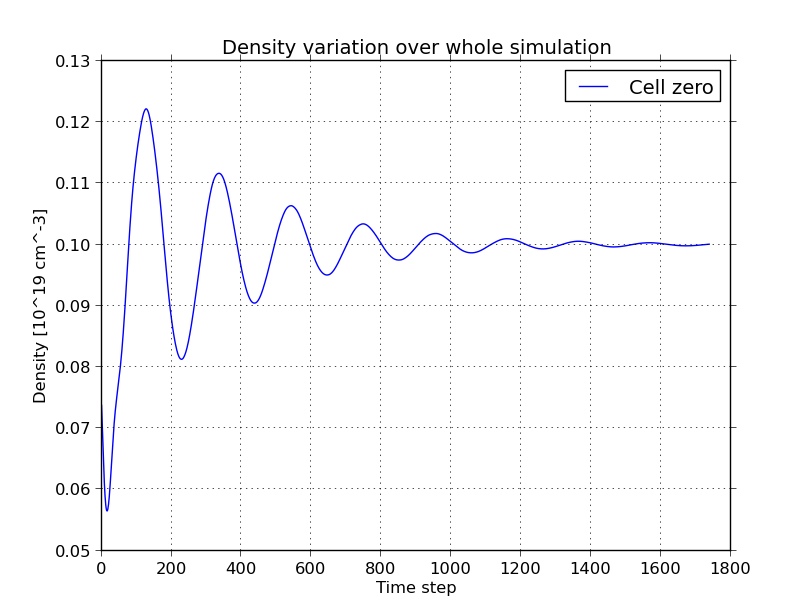
\includegraphics[scale=0.4]{Figures/sol1d/ne_var_ny=800.png}
\centering
\caption{The variation of \neus with simulation time step. \textbf{should maybe put the oscillations from other resolutions on the same figure to make it more interesting?}}\label{figne_var_ny=800}
\end{figure}

An important first step when running grid simulations is to ascertain an acceptable resolution to use. Figure~\ref{figRE_neres1000} shows the approximate steady-state value of \netarget for different resolutions. The choice of resolution has to take into account the accuracy of the output and the time taken to receive said output. It is clear that \netg is tending towards a value at infinite resolution. There is a 5.0\% change from 200 to 400 cells, 1.6\% change from 400 to 600, 0.58\% change from 600 to 800 cells and a 0.42\% change from 800 to 1000 cells. Given that the number of operations performed by the code scales as approximately $N^2$ for $N$ cells, increasing the cell number heavily increases the computing cost. Table~\ref{tabsol1dres} contains run times at different resolutions, and shows a stark increase in time for increasing resolution. The second run, at \neus $= 1.25\e{19}$ cm$^{-3}$, completed significantly faster than the first run because it was restarted from the near steady-state snapshot at the end of the first run. Therefore, each simulation time step is completed faster because the system is already rather stable, and only needs to accommodate an injection of an extra $0.25\e{19}$ cm$^{-3}$ of material in from the upstream.

\begin{table}[]
%\centering
\caption{SOL1D simulation run times and percentage change in }
\label{tabsol1dres}
\begin{tabular}{l|l|l|l|l|l}
\multicolumn{1}{l|}{\multirow{2}{*}{}} & \multicolumn{3}{l}{Time taken to complete 1000 time steps}    \\ \cline{2-3} 
 \multicolumn{1}{l|}{Resolution}        & \multicolumn{1}{l|}{\neus = $1.0$} & \multicolumn{1}{l|}{\neus = $1.25$}  & \netg & \% change  \\ \hline
                   200                 &      47m 44s          &    24m 23s         &  put    &  -    \\
                   400                 &      1h 48m 55s       &    2h 45m 4s       &  values & 5.0   \\
                   600                 &      7h 40m 57s       &    5h 5m 4s        &  in     & 1.6   \\
                   800                 &      13h 18m 55s      &    7h 1m 28s       &  here   & 0.58  \\
                  1000                 &                   &                        & *value* & 0.42
\end{tabular}
\end{table}

\begin{figure}
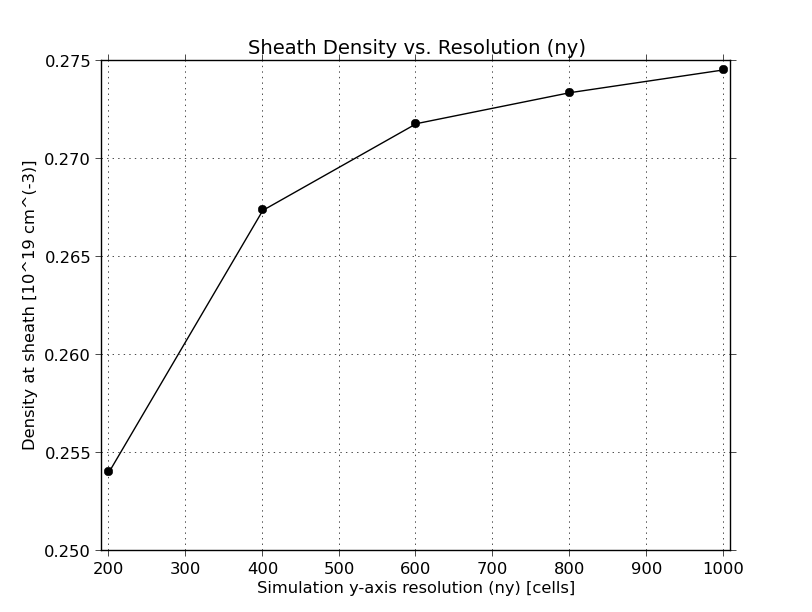
\includegraphics[scale=0.48]{Figures/sol1d/RE_neres1000.png}
\centering
\caption{Density at sheath, \netg, at approximately steady-state for different y-axis resolutions in SOL1D.}\label{figRE_neres1000}
\end{figure}

Detachment can be seen occurring when examining the density profiles of different simulations, figure~\ref{figneprofneusALLtriang} shows systems in varying states of detachment caused by differing set upstream densities. Although the precise point at which an attached system becomes detached can be debated. Panel a) shows an attached system, and even the higher resolution cases struggle to resolve the density profile close to the target, which is why the profiles are very jagged. Panel b) displays a detached system: the density profile peak has shifted away from the target plate somewhat, cooling the divertor surface. The density profile in panel c) is also detached from the target, but more so than in panel b), as although the profile shape adjacent to the target is a similar shape the peak has shifted toward the upstream. Once the density profile has retreated from the target it is much more easily resolved, as the peak is spread over many more cells than when it sits close to the surface. However, the low resolution case, with 200 cells along the y-axis, still struggles to produce a smooth profile close to the plate even when the system is quite detached. 

\begin{figure}
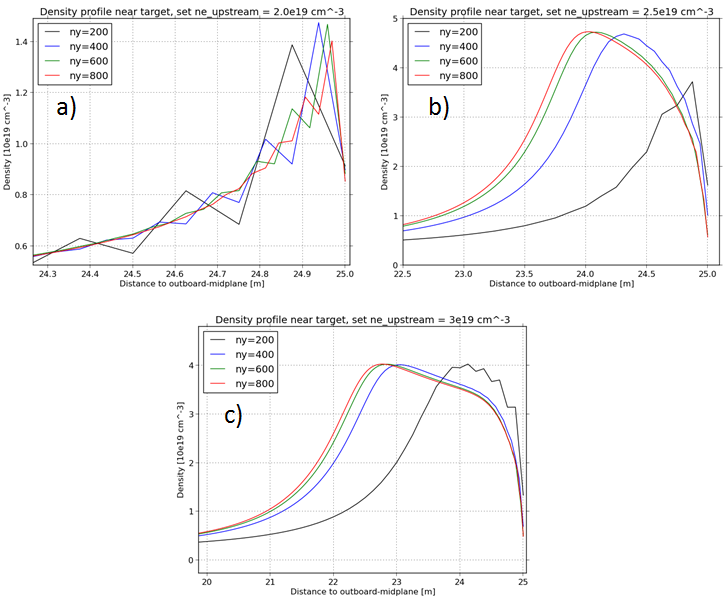
\includegraphics[scale=0.5]{Figures/sol1d/neprofneusALLtriang.png}
\centering
\caption{Density profile close to target for y-axis resolutions 200, 400, 600 \& 800 cells at different set values of \neus in SOL1D.}\label{figneprofneusALLtriang}
\end{figure}

These density profiles in figure~\ref{figneprofneusALLtriang} provide further evidence of the necessity of using a high enough resolution in grid-based simulations. The difference between the red (800 y-axis cells) and green (600) profiles is small compared to that with blue (400) or black (200), hence a resolution of 600 cells along the y-axis seems to attain sufficiently accurate results. Unless otherwise stated, subsequent SOL1D results were taken from simulations with ny = 600 cells.

\subsubsection{Temperature comparison}\label{sssectempcomp}
Two key parameters to be analysed are the upstream and target temperatures, \Tus and \Ttg. The whole point of divertor detachment is to reduce the power flux impacting on the divertor. \Ttg sets the voltage across the sheath, which in turn influences the velocity of ions impacting on the solid divertor target (ions in the simulation have a fixed velocity when entering the sheath - the Bohm velocity). The lower \Ttg, the less damage will be done to the divertor plates. Figure~\ref{figTT_IMPCOMBO2} shows the difference between \Tus and \Ttg for different \neus values at each of the resolutions in table~\ref{tabsol1dres}. When looking to reduce \Ttg, the trade off is the corresponding fall in \Tus. As the upstream is at the SOL midplane, any changes there will be translated directly into the main plasma. 

Similarly shaped temperature profiles are observed for all resolutions in figure~\ref{figTT_IMPCOMBO2}, \Tus falls slowly while \Ttg falls rapidly with increasing \neus, until above $2.25\e{19}$ cm$^{-3}$ when it starts to fall extremely fast. At this point, the density profile has pulled away from the divertor and this extra density flooding into the upstream is reducing the temperature there. If an operational 'sweet-spot' exists, then it is in the range $2\e{19}$ cm$^{-3}$ < \neus < $2.25\e{19}$ cm$^{-3}$, as here \Ttg has practically reached it's lower limit while \Tus is still quite high.

\begin{figure}
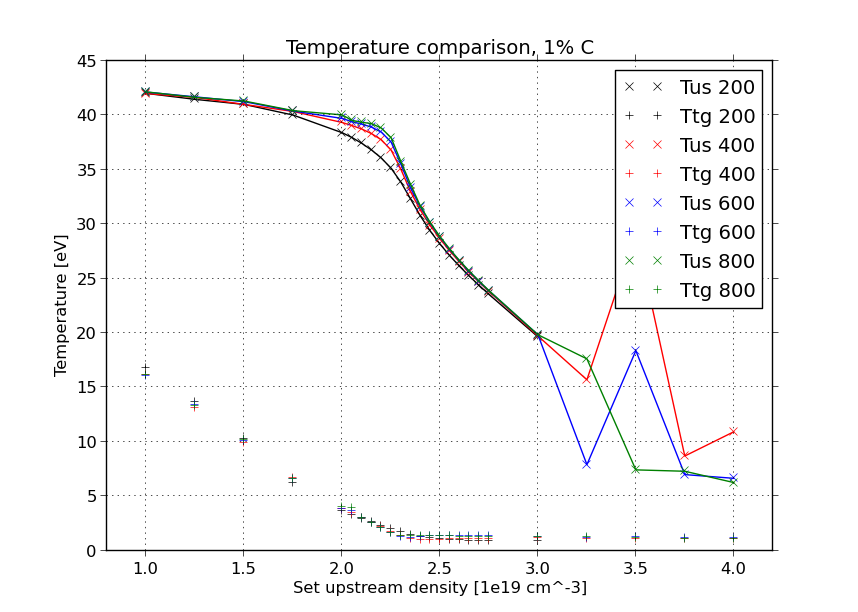
\includegraphics[scale=0.5]{Figures/sol1d/TT_IMPCOMBO2.png}
\centering
\caption{Comparison of $T_{upstream}$ and $T_{target}$ at varying set $n_{e~upstream}$ for different y-axis resolutions in SOL1D}\label{figTT_IMPCOMBO2}
\end{figure}

Simulations from \noNe{3} onwards shown in figure~\ref{figTT_IMPCOMBO2} are detaching and reattaching in quick succession, so they are unlikely to approach a steady state within a reasonable number of timesteps. When detached, the upstream temperatures in these simulations follow the downward trend observed with increasing \neus. However, when the system destabilises and rushes to reattach to the target plates, the upstream temperature shoots up. If these higher density simulations are terminated during a period of detachment, \Tus will be low, as is the case for all the \noNe{3.75} runs. Conversely, if they are terminated when the density profile has reattached, \Tus will be much higher, which can be seen in the data points at \noNe{3.5} for ny = 400 \& 600 cells. This cyclical detachment and reattachment is portrayed in figure~\ref{figny400800r35netg} - here \netg is observed following a pattern of peaks (when system is attached to the target) and troughs (when the system is detached). In the case of the black line, with y-axis resolution of 400 cells, the simulation has completed when the sheath density is still far higher than its minimum value, so the density profile is still in the process of detaching from the target surface. Consequently, the upstream temperature is still relatively quite high. The red line is from a simulation with the same input values but using 800 cells along the y-axis, here termination has occurred when the density profile is almost fully detached from the target, hence the upstream temperature is quite low. This termination snapshot effect can be seen in figure~\ref{figTT_IMPCOMBO2} at \noNe{3.5}, where the upstream temperature with 400 cells is much higher than that for 800 cells.

\begin{figure}
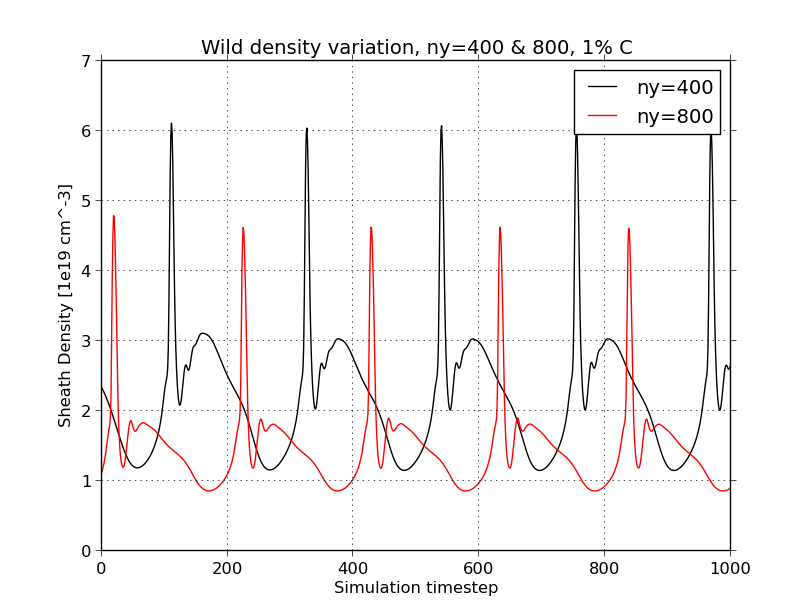
\includegraphics[scale=0.5]{Figures/sol1d/ny400800r35netg.png}
\centering
\caption{Continual detachment and reattachment causes the target $n_e$ variations for ny = 400 and 800 cells run with \neus~set to \noNe{3.5}.}\label{figny400800r35netg}
\end{figure}


\subsubsection{Pressure Loss}\label{sssecPloss}
Pressure ratio $2\frac{P_{tg}}{P_{us}}$ was calculated for the density scan data with different resolutions and plotted against target plate temperature in figure~\ref{figPL_IMPCOMBO2logy}; the data from varied resolutions show good agreement. Experimentally, pressure loss ratio saturates to unity at high target temperatures due to the relation between static and viscous (?) pressure (maths is on p18 of lab book) and falls as \Ttg decreases after the system has started to detach. Experimental pressure loss data is displayed in figure~\ref{figPlossAlcator}. The sharp drop in pressure loss ratio below 3 eV is thought to be caused by atomic effects which become relevant at those lower temperatures \cite{Pitcher1997}.

Pressure loss saturation is not observed in the simulations shown in figure~\ref{figPL_IMPCOMBO2logy}, and this discrepancy is expected to be due to the way ion viscosity is handled in the system. Ion viscosity varies like $\eta_i \propto \tau_i T \propto T^(\frac{5}{2}$, where $\tau_i$ is the ion collision time, hence this term in the overall viscosity equation is likely to blow up at higher temperatures, which would lead to the lack of saturation seen here. 

\begin{figure}
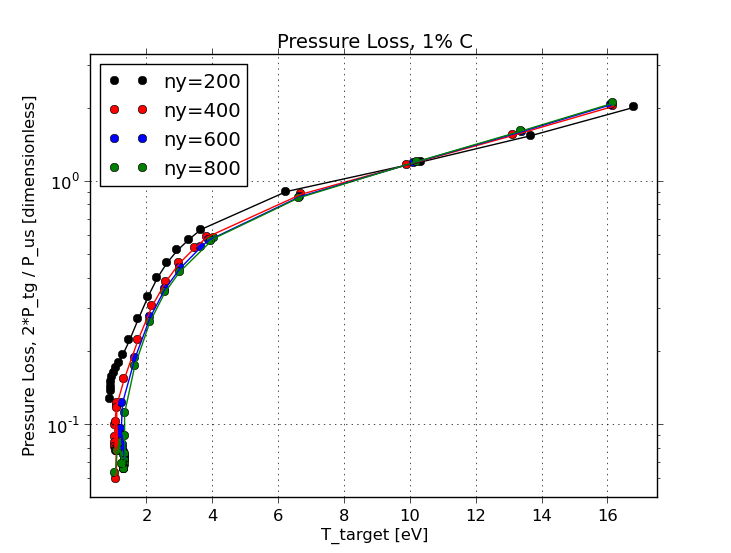
\includegraphics[scale=0.5]{Figures/sol1d/PL_IMPCOMBO2logy.png}
\centering
\caption{Pressure loss ratio, $\frac{2P_{tg}}{P_{us}}$, change with \Ttg at different y-axis resolutions in SOL1D.}\label{figPL_IMPCOMBO2logy}
\end{figure}

\begin{figure}
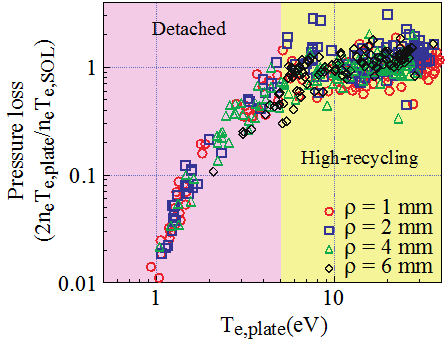
\includegraphics[scale=0.7]{Figures/PlossAlcator.png}
\centering
\caption{Pressure loss ratio, $\frac{2P_{tg}}{P_{us}}$, data from Alcator C-Mod \cite{Lipschultz2007}.}\label{figPlossAlcator}
\end{figure}



\subsubsection{Radiated Power}\label{sssecRpower}
SOL1D considers three types of radiated power: radiation due to impurities, Rzrad; due to ionisation, Riz and due to recombination, Rrec, which are combined to give total radiated power, R. An interesting quantity calculated from these three sources is the radiated power flux at a given time point in a simulation. This is given in equation~\ref{eqRpflux}, where $e$ is the charge of an electron, $\omega_{ci}$ is the ion cyclotron frequency, $dy$ is the simulation cell spacing and $\hat{N}$ and $\hat{T}$ are constants in the simulation given in the appendix. 

\begin{equation}\label{eqRpflux}
\hat{P}/A = (R~e~\hat{N}~\hat{T}~\omega_{ci}) \times dy
\end{equation}

\begin{figure}
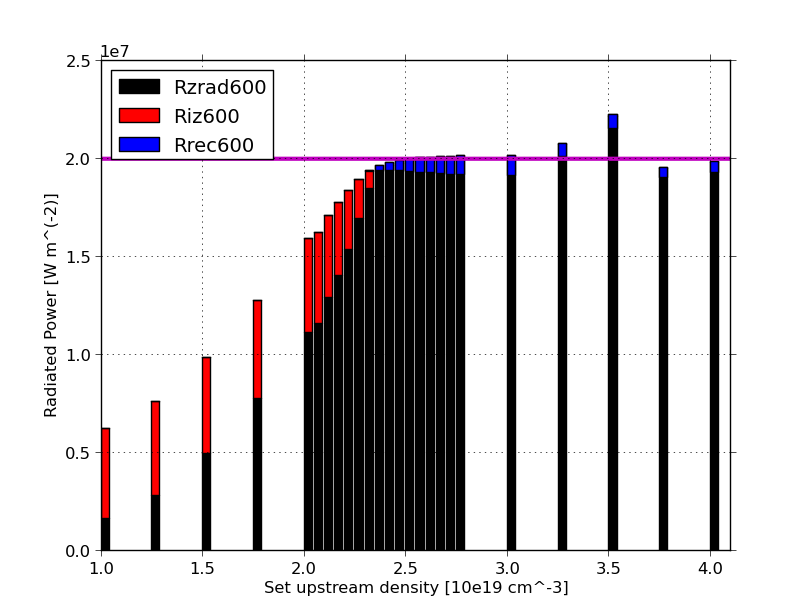
\includegraphics[scale=0.5]{Figures/sol1d/PRbar600.png}
\centering
\caption{Different sources of radiated power at varying set upstream density in SOL1D, with ny = 600 cells. The horizontal line shows the power flux entering the system.}\label{figPRbar600}
\end{figure}

Radiated power flux as a fraction of power flux input is expected to be lower at smaller values of \neus because system temperature is higher overall, and most species are fully ionised. This is observed in figure~\ref{figPRbar600}, as well as the expected radiated power increase as \neus increases and the system undergoes detachment, reducing the average temperature. As the temperature falls, more species begin to recombine, especially carbon initially. This is why an increase in radiation due to impurities, Rzrad, is observed up to a density of \noNe{2.5}, because carbon can recombine at higher temperatures than the other plasma species, providing significant power loss via Bremsstrahlung and energy level transitions.

Several of the higher \neus instances in figure~\ref{figPRbar600} show the system radiating more power than it receives. Neutrals formed in SOL1D come off the walls with a certain energy which is then transferred to the plasma. Hence, if enough neutrals transfer their energy to the plasma in one time step, the total power radiated can exceed the power input.

\subsubsection{Super-X Geometry}\label{sssecSXG}
Until now, the SOL1D simulations performed have used an arbitrary geometry and parameters (25m long field line and uniform B-field). Future simulations aim to emulate behaviour of MAST-Upgrade, which has just installed a Super-X divertor (SXD) in place of it's previous conventional divertor (CD); the differences between the two can be seen in figure~\ref{figCDvsSXD}. In the SXD geometry, the distance from the X-point to the target is much longer than the CD set up. Additionally, extra magnetic coils have been added into the nose of the bulkhead seen extending towards the X-point, which further separate the cold divertor plasma from the bulk plasma. These factors allow a greater tolerance when implementing conditions to achieve detachment, as changes in the divertor region are not transmitted as quickly or with the same magnitude as with the CD geometry.

\begin{figure}
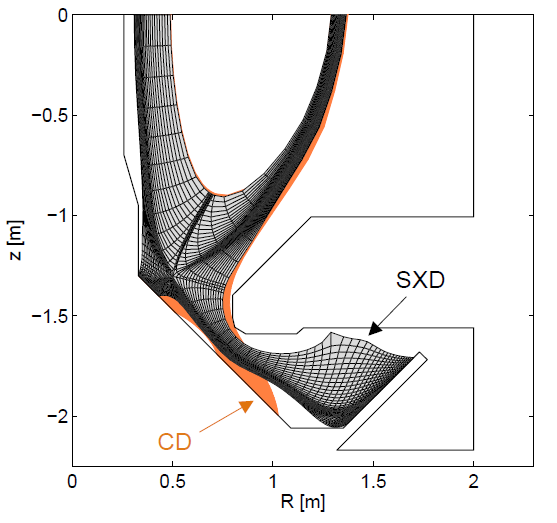
\includegraphics[scale=0.5]{Figures/CDvsSXD.png}
\centering
\caption{A comparison of the Super-X Divertor (SXD) and the Conventional Divertor (CD) geometries on MAST \cite{Havlickova2014}.}\label{figCDvsSXD}
\end{figure}

Implementing this new geometry requires estimating how the magnetic field changes over the length of the field line. This is entered into the simulations by changing the Area Expansion Ratio (AER), which describes how the cross section of a flux tube changes as it traverses the length of the field line. A distance of $0.05$ m out from the separatrix into the SOL was used, thus by using the third panel in figure~\ref{figMASTUdesignpapersFig2} the AER is estimated to be 12. Furthermore, the connection length of the field line between the X-point and the target is estimated as $26$ m, from the second panel. The connection length between the outboard midplane and the X-point is $5$ m \cite{Fishpool2013}, making the total length of the simulation y-axis $31$ m.

\begin{figure}
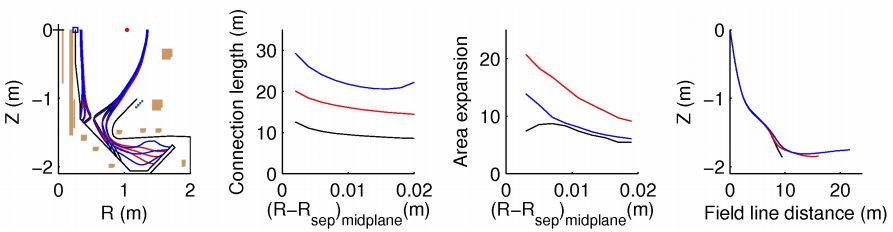
\includegraphics[scale=0.55]{Figures/MASTUdesignpapersFig2.png}
\centering
\caption{Representative magnetic equilibria with full toroidal field (0.8T vacuum at R=0.8m) showing conventional (black), expanded strike point (red) and Super-X like long connection length (blue) divertor geometries on MAST \cite{Fishpool2013}. \textbf{add in lines at 0.005 m to make the choice of Connection Length and Area Expansion v obvious.}}\label{figMASTUdesignpapersFig2}
\end{figure}


\subsubsection{Ion Viscosity}\label{sssecIonviscosity}
To study the lack of saturation at higher \Ttg values, seen in figure~\ref{figPL_IMPCOMBO2logy}, simulations were run neglecting ion viscosity, $\eta_i$, in the system. As discussed in section~\ref{sssecPloss}, $\eta_i$ varies as $T^{5/2}$ so may blow up at high temperatures. When removing the effects of ion viscosity, the saturation observed experimentally is seen in the simulation data, which is shown in figure~\ref{figPL_iVpts}. Ignoring ion viscosity results in higher average ion velocity in the target area and hence higher target temperature, which is the drawback to removing these effects from the system. Another drawback is that these simulations take significantly longer to reach near steady-state conditions, as ion viscosity is a large contributor to damping in the system.

A possible method of retaining the pressure loss saturation alongside viscous ion properties would be to introduce a flux limiter into the SOL1D framework. The current heat flux model \cite{Braginskii1965} fails to get close to the real value at high temperature gradients, because it approximates heat flux as varying linearly with $\nabla T$ which misses the asymptote at $q_max$. This limit exists because heat in a system cannot flow faster than the electron thermal velocity in that system.

\begin{figure}
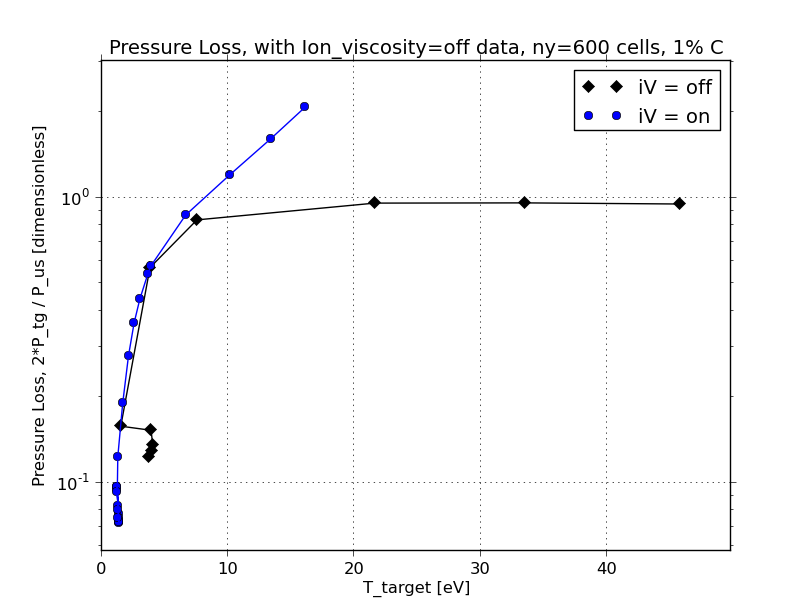
\includegraphics[scale=0.5]{Figures/sol1d/PL_iVpts.png}
\centering
\caption{Pressure loss data with and without the effects of ion viscosity, $\eta_i$, the inclusion of which prevents pressure loss saturation at higher \Ttg.}\label{figPL_iVpts}
\end{figure}

Free-streaming, or Spitzer Harm, thermal conductivity provides a better model of plasma heat flow, and is implemented in the Hermes 2D code. \textbf{trying to port this into sol1d}

The extended divertor leg in the SXD geometry enables simulations to settle down far quicker than in the CD set up, as the power input (at the midplane) is much farther removed from the complicated and delicately balanced interactions at the target. 




\section{Conclusion}\label{secConclusion}

- Applicability of Detachment in areas other than fusion: Coronal Loops exhibiting detachment (need to flick through the 2 papers I have on this topic) 
Prominences: A. De Groof, et al, A\&A 443, 319–328 (2005)
Coronal Rain: P. Antolin et al, 280 (2012) 457.





\printbibliography

\end{document}
